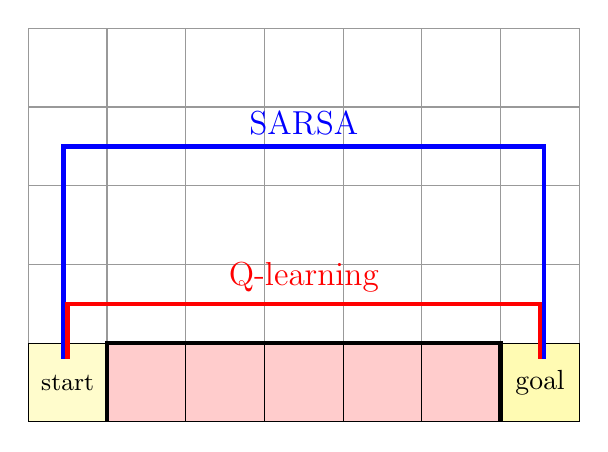
\begin{tikzpicture}[ node distance =1.3cm, > =  stealth, hv path/.style={to path={-| (\tikztotarget)}}, vh path/.style={to path={|- (\tikztotarget)}}]

\foreach \x in {1,...,7} 
{
	\foreach \y in {2,...,5} 
	{
	\node [rectangle, draw, minimum size = 1cm, black!40] at (\x,\y) {};
	}
}
\node [rectangle, draw, minimum size = 1cm, fill = yellow!20] at (1,1) {};
\node at (1,1) {\small{start}};
\node [rectangle, draw, minimum size = 1cm, fill = yellow!30] at (7,1) {goal};
\foreach \x in {2,...,6} 
	{
	\node [rectangle, draw, minimum size = 1cm, fill = red!20] at (\x,1) {};
	}
%cliff border	
\draw [ultra thick] (1.5, 0.5) -- (1.5,1.5) -- (6.5,1.5) -- (6.5,0.5);
%SARSA path
\draw [ultra thick, blue] (0.95,1.3) -- (0.95,4) -- node[midway, above] {\large{SARSA}} (7.05,4) -- (7.05,1.3);
%Q-learning path
\draw [ultra thick, red] (1,1.3) -- (1,2) -- node[midway, above] {\large{Q-learning}} (7,2) -- (7,1.3);
\end{tikzpicture}